\begin{abox}
	Assignment-S02\\
	\vspace{0.5cm}
	 Electrostatic Energy, Conductors and Electric Dipole
	\end{abox}
\begin{enumerate}
	\item $\left. \right. $
	\begin{answer}
		\begin{align*}
		\text{Electrostatic energy in spherical shell }W_{\text {shell }}&=\frac{\varepsilon_{0}}{2} \int_{0}^{R}\left|\vec{E}_{1}\right|^{2} 4 \pi r^{2} d r+\frac{\varepsilon_{0}}{2} \int_{R}^{\infty}\left|\vec{E}_{2}\right|^{2} 4 \pi r^{2} d r\\
		 \Rightarrow W_{\text {shell }}&=\frac{\varepsilon_{0}}{2} \int_{R}^{\infty} \frac{q^{2}}{\left(4 \pi \varepsilon_{0}\right)^{2} r^{4}} 4 \pi r^{2} d r\\&=\frac{q^{2}}{8 \pi \varepsilon_{0}}\left(-\frac{1}{r}\right)_{R}^{\infty}=\frac{q^{2}}{8 \pi \varepsilon_{0}} \frac{1}{R}\\
		\text{Electrostatic energy in solid sphere }W_{\text {solid sp }}&=\frac{\varepsilon_{0}}{2} \int_{0}^{R}\left|E_{1}\right|^{2} 4 \pi r^{2} d r+\frac{\varepsilon_{0}}{2} \int_{R}^{\infty}\left|E_{2}\right|^{2} 4 \pi r^{2} d r\\
		 \Rightarrow W_{\text {solid } s p}&=\frac{q^{2}}{8 \pi \varepsilon_{0}} \times \frac{1}{R^{6}}\left[\frac{r^{5}}{5}\right]_{0}^{R}+\frac{q^{2}}{8 \pi \varepsilon_{0}}\left[-\frac{1}{r}\right]_{R}^{\infty}\\&=\frac{q^{2}}{5 \times 8 \pi \varepsilon_{0}} \cdot \frac{1}{R}+\frac{q^{2}}{8 \pi \varepsilon_{0} R}=\frac{6 q^{2}}{40 \pi \varepsilon_{0} R}\\
		\text{Now }\frac{W_{\text {shell }}}{W_{\text {solid sp }}}&=\frac{\frac{q^{2}}{8 \pi \varepsilon_{0}}}{\frac{6 q^{2}}{40 \pi \varepsilon_{0} R}}=\frac{5}{6}
		\end{align*}
	\end{answer}
\item $\left. \right. $
\begin{answer}
	\begin{align*}
V&=\frac{q}{4 \pi \varepsilon_{0} R}\text{ and }W=\frac{q^{2}}{8 \pi \varepsilon_{0} R}.\\
	\text{Thus }W&=\frac{\left(4 \pi \varepsilon_{0} V R\right)^{2}}{8 \pi \varepsilon_{0} R}=\frac{4 \pi \varepsilon_{0} V^{2} R}{2}\\&=\frac{900 \times 10^{-2}}{9 \times 10^{9} \times 2}=0.5 \times 10^{-9}=5 \times 10^{-10} \mathrm{Joules}
	\end{align*}
\end{answer}
\item $\left. \right. $
\begin{answer}
	\begin{align*}
	\vec{E}&=\frac{Q}{4 \pi \varepsilon_{0} r^{2}} \hat{r} ; r>R\text{ and }\vec{E}=0 ; r<R\\
	W&=\frac{\varepsilon_{0}}{2} \int_{0}^{R} E_{1}^{2} 4 \pi r^{2} d r+\frac{\varepsilon_{0}}{2} \int_{R}^{\infty} E_{2}^{2} 4 \pi r^{2} d r \Rightarrow U=\frac{Q^{2}}{8 \pi \varepsilon_{0} R} \\
	\Rightarrow U^{\prime}&=\frac{(2 Q)^{2}}{8 \pi \varepsilon_{0} \frac{R}{2}}=\frac{8 Q^{2}}{8 \pi \varepsilon_{0} R}=8 U
	\end{align*}
\end{answer}
\item $\left. \right. $
\begin{answer}
		 Work done in placing first charge ( $q$ charge upper left corner) $W_{1}=0$\\
	Work done in placing second charge ( $2 q$ charge lower left corner) $W_{2}=\frac{1}{4 \pi \varepsilon_{0}}\left(\frac{2 q^{2}}{a}\right)$\\
	Work done in placing third charge ( $3 q$ charge lower right corner)
	\begin{align*}
	W_{3}&=\frac{1}{4 \pi \varepsilon_{0}}\left(\frac{6 q^{2}}{a}+\frac{3 q^{2}}{\sqrt{2} a}\right)
\intertext{	Potential at fourth corner ( $4 q$ charge upper right corner)}
	V&=\frac{1}{4 \pi \varepsilon_{0}} \sum \frac{q_{i}}{r_{i}}=\frac{1}{4 \pi \varepsilon_{0}}\left(\frac{q}{a}+\frac{2 q}{\sqrt{2} a}+\frac{3 q}{a}\right)\\&=\frac{q}{4 \pi \varepsilon_{0} a}(4+\sqrt{2}) \Rightarrow W_{4}=4 q V=\frac{4 q^{2}}{4 \pi \varepsilon_{0} a}(4+\sqrt{2})
\intertext{	Total work done}
W&=W_{1}+W_{2}+W_{3}+W_{4}=\frac{1}{4 \pi \varepsilon_{0}}\left(\frac{2 q^{2}}{a}\right)+\frac{1}{4 \pi \varepsilon_{0}}\left(\frac{6 q^{2}}{a}+\frac{3 q^{2}}{\sqrt{2} a}\right)+\frac{4 q^{2}}{4 \pi \varepsilon_{0} a}(4+\sqrt{2})\\
\Rightarrow W&=\frac{q^{2}}{4 \pi \varepsilon_{0} a}\left[2+\left(6+\frac{3}{\sqrt{2}}\right)+4(4+\sqrt{2})\right]\\&=\frac{q^{2}}{4 \pi \varepsilon_{0} a}\left[24+\frac{11}{2} \sqrt{2}\right]=\frac{q^{2}}{8 \pi \varepsilon_{0} a}\left[24+\frac{11}{2} \sqrt{2}\right]
	\end{align*}
\end{answer}
\item $\left. \right. $
\begin{answer}
	\begin{align*}
\text{(a) }\sigma_{a}&=0, \sigma_{b}=0, \sigma_{c}=0\text{ and }\sigma_{d}=\frac{+q}{4 \pi d^{2}}.\\
	\text{(b) }\sigma_{a}&=0, \sigma_{b}=\frac{+q}{4 \pi b^{2}}, \sigma_{c}=\frac{-q}{4 \pi c^{2}}\text{ and }\sigma_{d}=\frac{+q}{4 \pi d^{2}}.\\
	\text{(c) }\sigma_{a}&=0, \sigma_{b}=\frac{+q}{4 \pi b^{2}}, \sigma_{c}=\frac{-q}{4 \pi c^{2}}\text{ and }\sigma_{d}=\frac{+2 q}{4 \pi d^{2}}.\\
	\text{(d) }\sigma_{a}&=\frac{+q}{4 \pi b^{2}}, \sigma_{b}=\frac{-q}{4 \pi b^{2}}, \sigma_{c}=\frac{+q}{4 \pi c^{2}}\text{ and }\sigma_{d}=\frac{-q}{4 \pi d^{2}}.\\
	\text{(e) }\sigma_{b}&=\sigma_{d} \Rightarrow \frac{q}{4 \pi b^{2}}=\frac{2 q}{4 \pi d^{2}} \Rightarrow d=\sqrt{2} b\\
	\end{align*}
\end{answer}
\item $\left. \right. $
\begin{answer}
	\begin{align*}
 V&=\frac{p \cos \theta}{4 \pi \varepsilon_{0} r^{2}}\text{ and }\vec{E}=\frac{p}{4 \pi \varepsilon_{0} r^{3}}(2 \cos \theta \hat{r}+\sin \theta \hat{\theta})\\
\text{	(a) }&\operatorname{At}(0, b, 0) ; \quad \theta=\frac{\pi}{2} \Rightarrow \vec{E}=\frac{p}{4 \pi \varepsilon_{0} b^{3}} \hat{\theta}=-\frac{p}{4 \pi \varepsilon_{0} b^{3}} \hat{z}\\
	\text{(b) }&\text{The electrostatic potential at $(b, 0,0)$ is }V(b, 0,0)=0 \quad \because \theta=\frac{\pi}{2}\\
	\text{(c) }&\operatorname{At}(0,0, b) ; \quad \theta=0 \Rightarrow \vec{E}=\frac{2 p}{4 \pi \varepsilon_{0} b^{3}} \hat{r}\\
	&\text{If a charge $q$ is kept at }(0,0, b), \vec{E}=\frac{2 q p}{4 \pi \varepsilon_{0} b^{3}} \hat{z}.\\
	\text{(d) }&\text{The work done in moving a charge $q$ from }(0, b, 0)\text{ to }(0,0, b)\\&
	 W=q[V(0,0, b)-V(0, b, 0)]=q\left[\frac{p}{4 \pi \varepsilon_{0} b^{2}}-0\right]=\frac{q p}{4 \pi \varepsilon_{0} b^{2}}\\
\text{	(e) }&\text{Electric flux through a spherical surface enclosing the origin is zero.}
	\end{align*}
\end{answer}
\item $\left. \right. $
\begin{answer}
	\begin{align*}
	\vec{p}&=p \hat{z} \quad\text{ and }\quad \vec{E}=-\vec{\nabla} V=\frac{p}{4 \pi \varepsilon_{0} r^{3}}(2 \cos \theta \hat{r}+\sin \theta \hat{\theta})\\&=\frac{1}{4 \pi \varepsilon_{0} r^{3}}[3(\vec{p} \cdot \hat{r}) \hat{r}-\vec{p}]\\
	\vec{E}&=\frac{1}{4 \pi \varepsilon_{0} r^{3}}\left[3(p \hat{z}) \cdot\left(\frac{x \hat{x}+y \hat{y}+z \hat{z}}{r}\right) \frac{\vec{r}}{r}-p \hat{z}\right]\\&=\frac{1}{4 \pi \varepsilon_{0} r^{3}}\left[\frac{3 p z}{r}\left(\frac{x \hat{x}+y \hat{y}+z \hat{z}}{r}\right)-p \hat{z}\right] \\
	\Rightarrow E_{x}&=\frac{1}{4 \pi \varepsilon_{0}} \frac{3 p x z}{r^{5}}, E_{y}=\frac{1}{4 \pi \varepsilon_{0}} \frac{3 p y z}{r^{5}} \text { and } E_{y}=\frac{1}{4 \pi \varepsilon_{0} r^{3}}\left[\frac{3 p z^{2}}{r^{2}}-p\right]
	\end{align*}
\end{answer}
\item $\left. \right. $
\begin{answer}$\left. \right. $
	\begin{figure}[H]
		\centering
		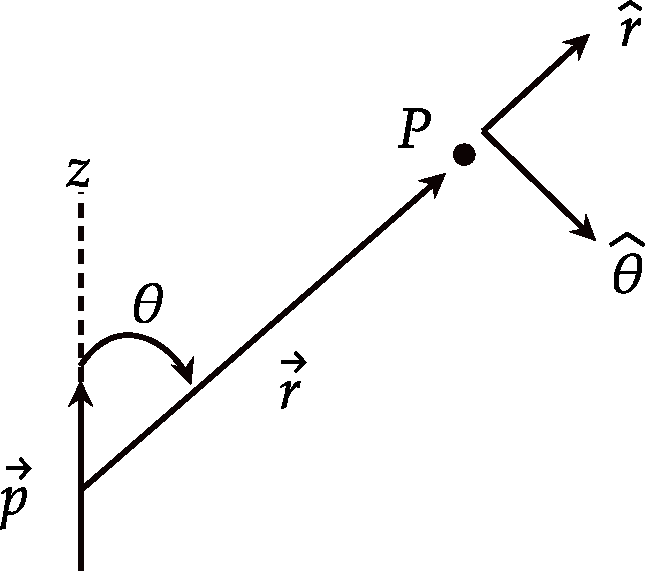
\includegraphics[height=3.5cm,width=4cm]{Assi-S10}
	\end{figure}
	\begin{align*}
	 \text{(a) }\vec{E}&=\frac{p}{4 \pi \varepsilon_{0} r^{3}}(2 \cos \theta \hat{r}+\sin \theta \hat{\theta}) \Rightarrow E_{r}=\frac{2 p \cos \theta}{4 \pi \varepsilon_{0} r^{3}}\text{ and }E_{\theta}=\frac{p \sin \theta}{4 \pi \varepsilon_{0} r^{3}}\\
	E_{z}&=E_{r} \cos \theta+E_{\theta} \cos (90+\theta) \\
	\Rightarrow E_{z}&=E_{r} \cos \theta-E_{\theta} \sin \theta=\frac{2 p \cos ^{2} \theta}{4 \pi \varepsilon_{0} r^{3}}-\frac{p \sin ^{2} \theta}{4 \pi \varepsilon_{0} r^{3}}=\frac{p}{4 \pi \varepsilon_{0} r^{3}}\left(3 \cos ^{2} \theta-1\right)\\
	\text{(b) }\vec{E}&=\frac{p}{4 \pi \varepsilon_{0} r^{3}}(2 \cos \theta \hat{r}+\sin \theta \hat{\theta}) \Rightarrow E_{r}=\frac{2 p \cos \theta}{4 \pi \varepsilon_{0} r^{3}}\text{ and }E_{\theta}=\frac{p \sin \theta}{4 \pi \varepsilon_{0} r^{3}}\\
	E_{\perp}&=E_{r} \sin \theta+E_{\theta} \sin (90+\theta) \\
	\Rightarrow E_{\perp}&=E_{r} \sin \theta+E_{\theta} \cos \theta=\frac{2 p \cos \theta \sin \theta}{4 \pi \varepsilon_{0} r^{3}}+\frac{p \sin \theta \cos \theta}{4 \pi \varepsilon_{0} r^{3}}=\frac{3 p \sin \theta \cos \theta}{4 \pi \varepsilon_{0} r^{3}}\\
	\text{(c) }\vec{E}&=\frac{p}{4 \pi \varepsilon_{0} r^{3}}(2 \cos \theta \hat{r}+\sin \theta \hat{\theta}) \Rightarrow E_{r}=\frac{2 p \cos \theta}{4 \pi \varepsilon_{0} r^{3}}\text{ and }E_{\theta}=\frac{p \sin \theta}{4 \pi \varepsilon_{0} r^{3}}\\
	\tan \alpha&=\frac{E_{\theta}}{E_{r}}=\frac{1}{2} \tan \theta\\
	\because \alpha&=90-\theta \Rightarrow \cot \theta=\frac{1}{2} \tan \theta \Rightarrow \tan ^{2} \theta=2 \Rightarrow \tan \theta=\sqrt{2}\\
	\Rightarrow \sin \theta&=\sqrt{\frac{2}{3}}\text{ and }\cos \theta=\frac{1}{\sqrt{3}}
	\end{align*}
	\begin{figure}[H]
		\centering
		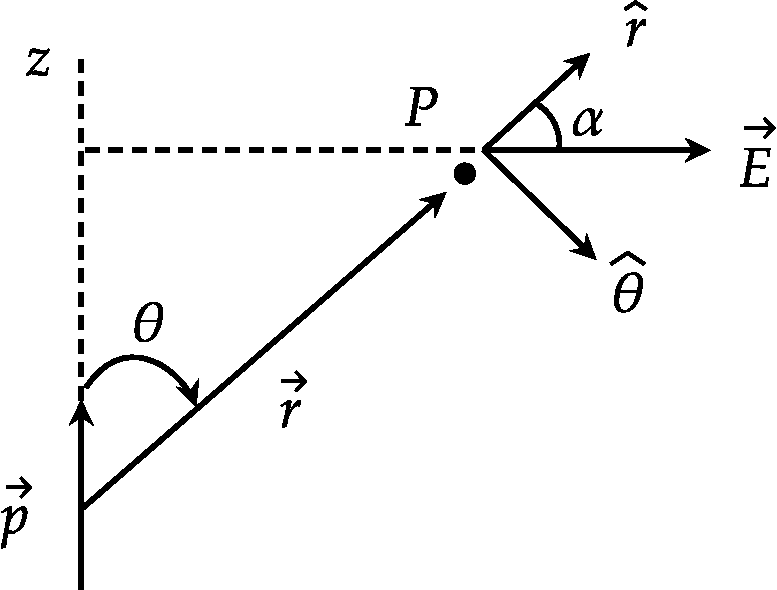
\includegraphics[height=3.5cm,width=4cm]{Assi-S11}
	\end{figure}
\end{answer}
\item $\left. \right. $
\begin{answer}
	\begin{align*}
	 \text{Electrostatic potential energy }U&=\frac{1}{4 \pi \varepsilon_{0} r^{3}}\left[\overrightarrow{p_{1}} \cdot \overrightarrow{p_{2}}-3\left(\overrightarrow{p_{1}} \cdot \hat{r}\right)\left(\overrightarrow{p_{2}} \cdot \hat{r}\right)\right]\\
	U \propto \frac{1}{r^{3}} \Rightarrow \frac{U_{2}}{U_{1}}&=\frac{r_{1}^{3}}{r_{2}^{3}}=\frac{1}{27}
	\end{align*}
\end{answer}
\item $\left. \right. $
\begin{answer}$\left. \right. $
	\begin{figure}[H]
		\centering
		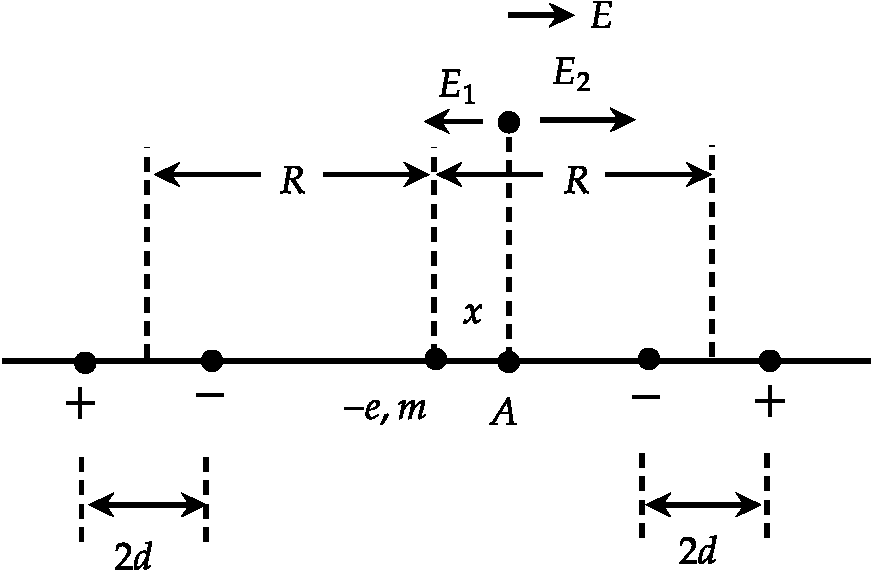
\includegraphics[height=4cm,width=6.5cm]{Assi-S12}
	\end{figure}
	Let us displace the charge particle by small amount $x$ at $A$.
	\begin{align*}
	\text{Field due to first dipole is }E_{1}&=\frac{2 p}{4 \pi \varepsilon_{0}} \frac{1}{(R+x)^{3}}.\\
	\text{Field due to second dipole is }E_{2}&=\frac{2 p}{4 \pi \varepsilon_{0}} \frac{1}{(R-x)^{3}}.
\intertext{	Then the resultant electric field at point $A$ is given by $E=E_{2}-E_{1} \quad \because E_{2}>E_{1}$}
	E&=\frac{2 p}{4 \pi \varepsilon_{0}}\left[\frac{1}{(R-x)^{3}}-\frac{1}{(R+x)^{3}}\right]=\frac{2 p}{4 \pi \varepsilon_{0} R^{3}}\left[\frac{1}{\left(1-\frac{x}{R}\right)^{3}}-\frac{1}{\left(1+\frac{x}{R}\right)^{3}}\right]\\&=\frac{2 p}{4 \pi \varepsilon_{0} R^{3}}\left[\left(1+3 \frac{x}{R}\right)-\left(1-3 \frac{x}{R}\right)\right] \\
	\Rightarrow E&=\frac{2 p}{4 \pi \varepsilon_{0} R^{3}}\left(6 \frac{x}{R}\right)=\frac{6 e d}{\pi \varepsilon_{0} R^{4}} x \quad \text { where } p=e \times 2 d=2 e d . \\
	F&=-e E=-\frac{6 e^{2} d}{\pi \varepsilon_{0} R^{4}} x=-k x\\
\text{	Then }\omega&=\sqrt{\frac{k}{2 m}}=\sqrt{\frac{6 e^{2} d}{2 \pi \varepsilon_{0} m R^{4}}}\\&=\sqrt{\frac{3 e^{2} d}{\pi \varepsilon_{0} m R^{4}}} \Rightarrow f=\frac{1}{2 \pi} \sqrt{\frac{3 e^{2} d}{\pi \varepsilon_{0} m R^{4}}}
	\end{align*}
\end{answer}
\end{enumerate}